% ===================================================================
% SKILL: SOSYAL MEDYA VE ETKİLEŞİM SAYFASI
% ===================================================================
% TANIM:
% Bu şablon, dersin sonlarına doğru veya iletişim bölümünde kullanılan,
% tüm sosyal medya kanallarını (YouTube, LinkedIn, Instagram) tek bir
% tam ekran görsel üzerinde toplayan, modern ve şık bir frame oluşturur.
% 
% ÖZELLİK:
% Görsel tam ekran arkaplan olarak yerleşir. Alt kısımda beyaz, şeffaf
% bir kutu içinde açıklama metni bulunur ("Overlay Text").
% ===================================================================

% "plain" ve "noframenumbering" ile sayfa numarası ve üst bilgiler gizlenir.
\begin{frame}[plain,noframenumbering]
    \begin{tikzpicture}[remember picture,overlay]
        % 1. TAM EKRAN GÖRSEL
        % Arka plana Combined QRs görselini yerleştirir.
        \node[anchor=center, at=(current page.center), inner sep=0pt] {
            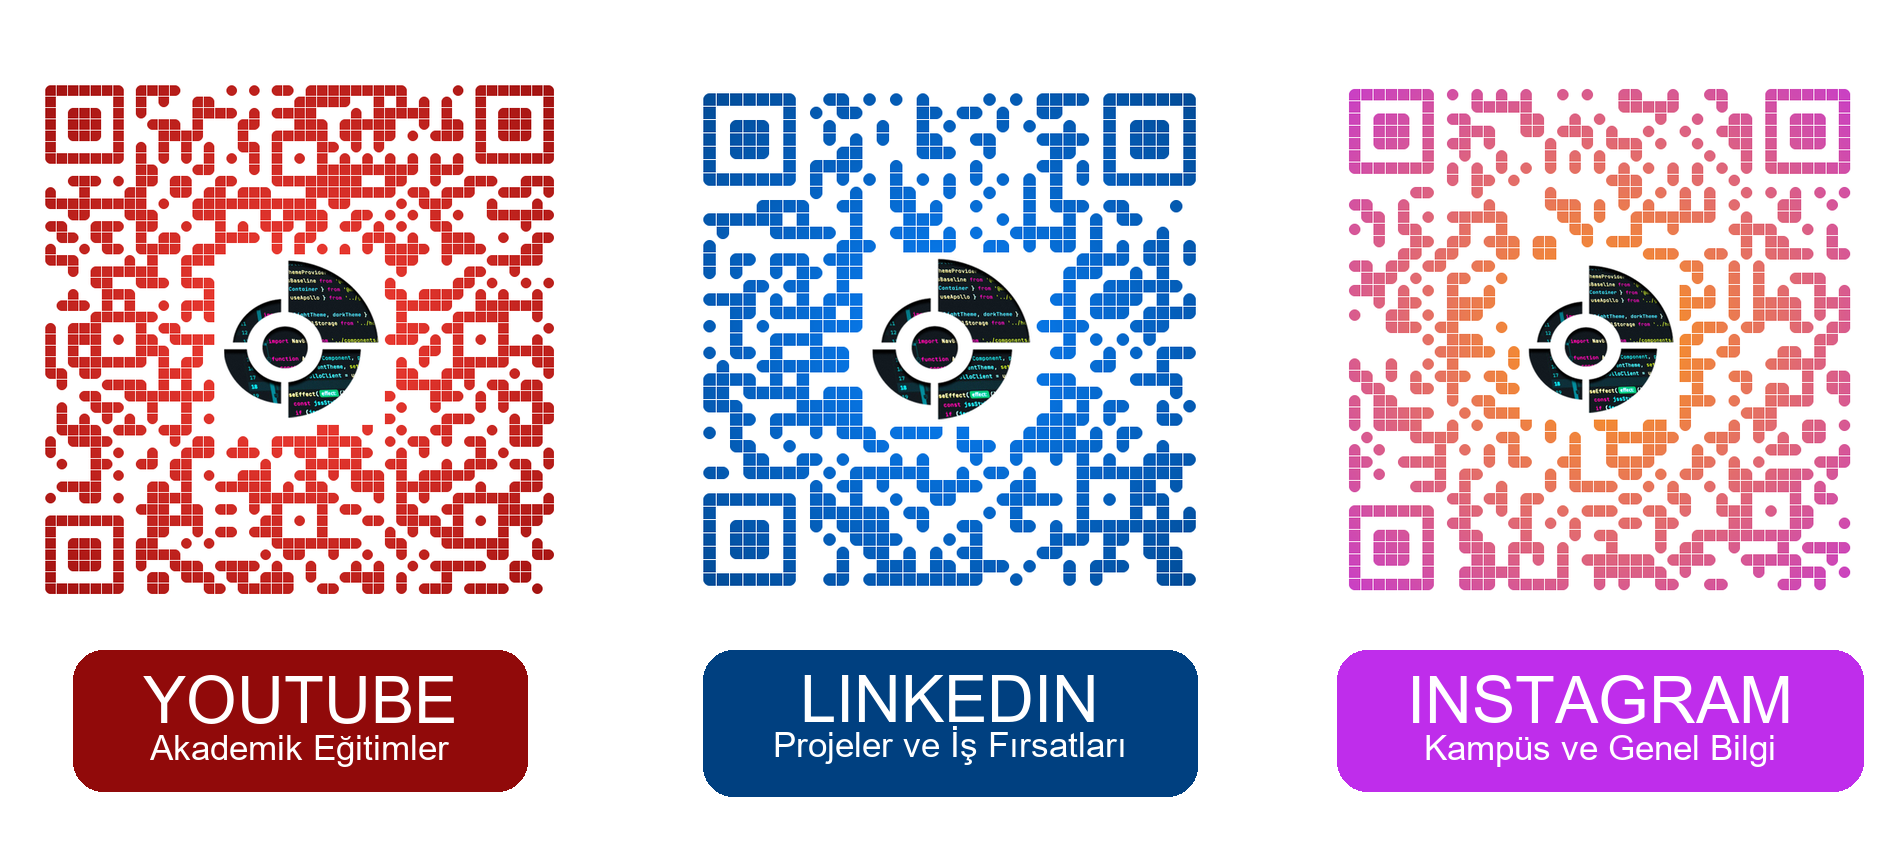
\includegraphics[width=\paperwidth, height=\paperheight]{figures/combined_qrs.png}
        };
        
        % 2. OVERLAY METİN (BEYAZ KUTU)
        % Görselin alt kısmına okunaklı bir mesaj kutusu ekler.
        \node[anchor=south, at=(current page.south), yshift=0.5cm, fill=white!95, rounded corners, inner sep=10pt, text width=0.95\paperwidth, align=center] {
            \Large \textbf{\textcolor{blue}{Bizi Takip Edin!}} \\
            \vspace{0.3em}
            \small Ders tekrarlarıyla konuları pekiştirmek (YouTube), profesyonel proje ağlarına katılmak (LinkedIn) ve kampüs duyurularından anında haberdar olmak (Instagram) için topluluğumuza katılın.
        };
    \end{tikzpicture}
\end{frame}
